\chapter{Diseño e implementación}
\noindent
La aplicación recopila información del usuario en distintas etapas. Se trata de una aplicación web que ejecuta código tanto en cliente como en servidor para obtener dicha información.
\begin{itemize}
    \item \textbf{Cliente}: Es la parte de la aplicación ejecutada en el navegador del usuario. Obtiene información del navegador mediante código JavaScript y lo envía al servidor de forma asíncrona.
    \item \textbf{Servidor}: En el se encuentra la base de datos y el código que obtiene la información de las cabeceras http y de las inserciones y actualizaciones de la base de datos.
     \begin{itemize}
         \item \textbf{Base de datos}: Una base de datos sencilla del tipo MySQL en la que se almacenarán los datos obtenidos de cada una de las conexiones de los usuarios.
     \end{itemize}
\end{itemize}
\section{Funcionamiento}
Nuestra aplicación se ejecuta tanto en cliente como en servidor, en distintas etapas y comunicándose de manera asíncrona en algunas de ellas. \par
El cliente hace una petición HTTP al servidor, de la cual el servidor analiza las cabeceras de la petición y las inserta en la base de datos con un identificador asociado al usuario para definir su huella. Devuelve al usuario una página estática en HTML con JavaScript embebido en la que el usuario verá los datos de su cabecera HTTP y el código JavaScript se ejecutará automáticamente para obtener el resto de datos del navegador. \par
Una vez terminada la ejecución de todo el código JavaScript este actualizará la apariencia de la página para que el usuario pueda ver también sus características obtenidas mediante JavaScript y enviará de forma asíncrona, sin recargar la página del usuario, toda la información obtenida al servidor. \par
El servidor recibe la información obtenida en JavaScript y actualiza todas las filas de las tablas de la base de datos para el id del usuario. \par
Por último el servidor ejecuta el código encargado de calcular la unicidad de cada uno de los atributos del usuario por separado y la unicidad total del conjunto de atributos. Tras calcularlo devolverá como respuesta de la petición asíncrona del código JavaScript todos los valores de la unicidad, que volverán a actualizar la página para mostrarle al usuario como de único es en cada uno de los campos de su navegador y como de único es su navegador en conjunto.
\begin{figure}[H]
    \centering
    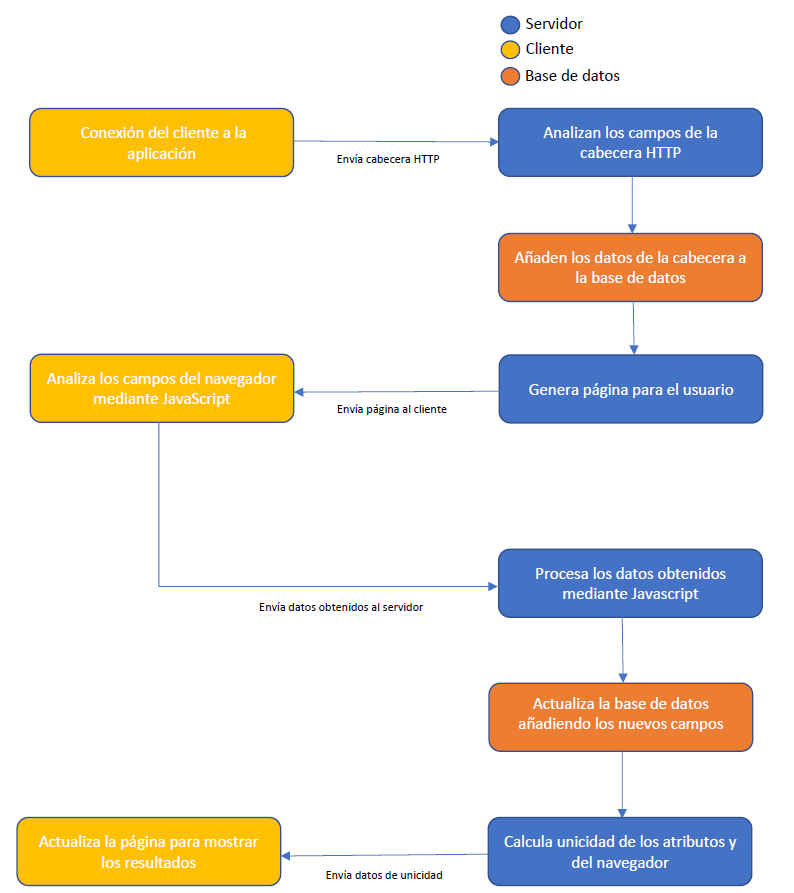
\includegraphics[width=0.7\textwidth]{Images/diagrama flujo.png}
    \caption{diagrama de flujo de la aplicación}
    \label{fig:diagramaFlujo}
\end{figure}
\section{Componentes del sistema}
El proyecto cuenta con distintos componentes, principalmente divididos en cliente y servidor.
\subsection{Servidor}
El servidor se encarga de gestionar las peticiones HTTP enviadas por el usuario al utilizar nuestra aplicación web.\par
La página consta de dos rutas, que serán generadas por el servidor mediante PHP:
\begin{itemize}
    \item \textbf{Página principal}: Es la base de la aplicación. En ella se analizan y muestran todos los elementos del navegador del usuario, así como su unicidad general e individual de cada uno de los atributos del navegador.
    \item \textbf{Página de gráficas}: En esta página se muestra al usuario gráficas con los datos globales de los atributos obtenidos por la aplicación.
\end{itemize}
Para la parte principal de la aplicación el servidor actúa en dos ocasiones.\par
La primera se encarga de recopilar la información de la cabecera HTTP, generar la página que verá el usuario y de insertar en la base de datos esta información.\par 
La segunda recibe una petición asíncrona con los datos obtenidos en la ejecución de código en cliente. El servidor se encarga de actualizar la base de datos añadiendo esos datos a las tablas para el id del usuario y una vez añadida esta información genera un objeto JSON que devolverá como respuesta de la petición y en el que se encuentra la unicidad de cada uno de los elementos analizados y la unicidad general del navegador del usuario.
\subsubsection{Lenguaje}
Para el código en servidor hemos utilizado el lenguaje PHP. Con el se gestiona todo el funcionamiento de la aplicación en el servidor.\par
En el servidor se generan las páginas HTML que se envían al cliente. Al ser necesario que cada cliente reciba una página única y personalizada estas se generan de manera dinámica en el servidor con este lenguaje. Por otra parte PHP nos permite obtener la información de la cabecera HTTP que recibe el servidor y tratarla para añadir esta información en la página que verá el cliente y a su vez insertarla en nuestra base de datos.\par
\subsubsection{Base de datos}
La base de datos de nuestra aplicación es de tipo MySQL. Consta de 6 tablas.
\subsection{Cliente}
En cliente se carga la página del usuario, en la que se muestran los datos del navegador en el que se está ejecutando la aplicación.\par
La página que recibe el usuario es dinámica. Al principio en ella se muestra la información obtenida de la cabecera HTTP mientras se ejecuta código JavaScript encargado de obtener el resto de datos del navegador. Cuando se termina de ejecutar esta parte se realiza una llamada asíncrona al servidor, en la que se envían todos los datos obtenidos y la página queda a la espera de la respuesta de este. Al recibir la respuesta, en la que se encuentran todos los valores de la unicidad del navegador, se actualiza la apariencia de la página para que el usuario pueda terminar de ver toda la información relacionada a su navegador y como de única es su huella. 
\subsubsection{Lenguaje}
El lenguaje utilizado en cliente es HTML para generar la página, con JavaScript para toda la parte dinámica.\par 
El código JavaScript se encarga de obtener datos del navegador mediante clases y funciones predefinidas en el JavaScript y otros métodos desarrollados por nosotros (añadir referencia a la sección de fuentes de información cuando esté todo escrito en latex). Además JavaScript nos permite realizar las peticiones asíncronas al servidor de forma que se puede actualizar la página sin necesidad de recargarla una vez recibe la respuesta del servidor.\par 
Para la generación de los gráficos de las estadísticas de la aplicación utilizamos la herramienta de <<Google Charts>>, la cual importamos mediante JavaScript y que permite crear distintos tipos de gráficas.
\subsection{Problemas}
Durante el desarrollo de la aplicación nos hemos encontrado con distintos problemas, los cuales detallaremos a continuación y las soluciones que hemos encontrado para estos.
\subsubsection{Asincronía}
Este problema surgió durante la implementación de la parte asíncrona de nuestra aplicación. Para la realización de esta utilizamos el objeto  <<XMLHTTPRequest>> de JavaScript. Este permite realizar peticiones al servidor mientras se sigue ejecutando código en cliente y, una vez recibe la respuesta del servidor, puede ejecutar funciones que estaban a la espera de la respuesta. El código JavaScript que utilizamos está dividido en distintas secciones, dependiendo de los objetos que se utilizan o el tipo de información que se obtiene. Una vez se termina de obtener todos los datos de cada sección se realiza el envío de información al servidor de esa parte. Solo en el último envío, cuando ya están todos los datos alojados en el servidor se espera la información devuelta por este para actualizar la página.\par 
Al ejecutarse el código de manera asíncrona en el servidor, en algunas ocasiones se ejecutaba la última petición antes que el resto, por lo que se retornaba una unicidad errónea del navegador, ya que se recibía la respuesta antes de que el resto de datos hubiesen sido añadidos en el servidor.\par 
Para solucionarlo hicimos que una vez lanzada una petición asíncrona no lanzase la siguiente hasta haber recibido la respuesta del servidor, de forma que se lanzasen síncronamente.
\subsection{Campos de cabeceras HTTP}
Los elementos de la cabecera HTTP puede variar de un navegador a otro, e incluso dentro del mismo navegador. Nuestra aplicación analiza todos los campos de la cabecera HTTP de manera automática, por lo que en ocasiones pueden aparecer elementos con los que no contamos.\par 
La solución fue analizar los elementos mas comunes a todos los navegadores y controlar que solo fuesen esos los que tratamos dentro de la aplicación. Esta comprobación la hacemos mediante PHP en el servidor. El resto de datos solo se muestran en la página al usuario para comprobar los elementos que conforman la cabecera HTTP de su navegador.
\subsection{Futuras mejoras}
Durante el trabajo hemos dejado funcionalidades o mejoras que se podrían realizar en el futuro para mejorar el desempeño de la aplicación.
\subsubsection{Asincronía}
En nuestra aplicación hemos utilizado el objeto <<XMLHTTPRequest>> de JavaScript para la conexión asíncrona con el servidor. Se trata de un objeto que empieza a estar obsoleto y que ha sido reemplazado por <<Fetch>>, que permite acceder y manipular partes del canal HTTP de manera mas sencilla y cómoda.\par 
Además se puede buscar una mejor solución al problema de la asincronía mencionado anteriormente.
\subsubsection{Gráficas}
Se puede realizar una modificación de la gráficas, de forma que al dibujarse estas se resalte la porción a la que pertenece el navegador del usuario que la está viendo.\par 
También se puede añadir una mejora que permita al usuario ver una nueva gráfica al seleccionar un campo de otra, en la que se detalle información de la anterior. Por ejemplo, en la gráfica de sistema operativo, al pulsar sobre uno de los sistemas se mostraría una nueva gráfica en la que se pudiese ver el porcentaje de cada una de las versiones de ese sistema.
\subsubsection{Analizar otros elementos del navegador}
Consideramos que nuestra aplicación obtiene información de suficientes elementos mediante JavaScript, pero durante el desarrollo dejamos varios por implementar por falta de tiempo. Entre ellos se podrían añadir los siguientes.
\begin{itemize}
    \item \textbf{WebGL}: Se trata de una API para JavaScript que permite renderizar gráficos en 3D. Se puede utilizar de forma similar a nuestra implementación de <<Canvas>>.
    \item \textbf{Sensores}: Mediante JavaScript se puede obtener información de sensores del dispositivo, como el acelerómetro o el giroscopio.
\end{itemize}